\section{Diskusjon}
I denne seksjonen av rapporten vil vi diskutere resultatene av eksperimentet og analysere dem i forhold til teorien og hensikten med studien. Vi vil også identifisere potensielle feilkilder, mulige bruksområder for funnene, og foreslå forbedringer og videre arbeid.

\subsection{Resultater knyttet til teori}
I denne seksjonen diskuterer vi resultatene for hver krets i forhold til teorien og forventningene basert på den idealiserte modellen av dioden og de faktiske karakteristiske kurvene. Det vil gjøres utregninger og fremstillinger for å understreke avvik og støtte teorien.



\paragraph{Krets 1 og 2 -- klippekrets. } Teorien for disse kretsen bygger på en idealisert modell av dioden, der den karakteristiske kurven tilnærmes som en loddrett linje ved $V_D = 0.7\text{V}$ som vist under.

\begin{figure}[H]
\centering
\begin{tikzpicture}
\begin{axis}[
    width=6cm,
    height=6cm,
    axis lines=middle,
    xlabel={$V_D[\text{V}]$},
    ylabel={$I_D[\text{mA}]$},
    xmin=0, xmax=1,
    ymin=0, ymax=10,
    xtick={0.7},
    xticklabels={$0.7$},
    ytick=\empty,
    grid=both,
    grid style={dashed, gray!30}
]

% Loddrett linje (ideal diode)
\addplot[
    red,
    very thick
] coordinates {
    (0.7, 0)
    (0.7, 10)
};

\end{axis}
\end{tikzpicture}
\caption{Teoretiske karakteristiske kurven til en diode.}\label{fig:idealisertKurveSilisium}
\end{figure}

\noindent
Denne modellen avviker fra hva den reelle karakteristiske kurven er. En teoretisk tilnærming av diodens reelle karakteristiske kurve er i figur~\ref{fig:silisiumsDiodeKurve}. Oscilloskopbilde vil derfor være annerledes fra det teoretiske og et slikt avvik i resultatet må forventes. Måleresultatene viser at signalet klippes ved  $800\text{mV}$ i begge kretser, altså høyere enn den teoretiske absoluttverdien på $0.7\text{V}$. Dette samsvarer med den faktiske karakteristiske kurven til dioden: når strømmen gjennom dioden øker, vil også spenningen over den øke. 
\\[1em]
Videre observeres det at utgangssignalet begynner å avvike fra inngangssignalet tidligere enn den idealiserte modellen tilsier. Dette skyldes at en praktisk diode begynner å lede gradvis før den når $0.7\text{V}$, i motsetning til den brå overgangen i den idealiserte modellen. Dette forklarer hvorfor den praktiske målingen begynner å avvike fra inngangssignalet ved en lavere spenning enn den teoretiske klippeverdien. For å videre understreke at klippeverdien er forventet høyere. Kan vi se på maksimalstrømmen gjennom kretsen. Vi benytter målte verdier fra oscilloskopet og Ohms lov for å beregne maksimalstrømmen gjennom dioden:
\[
\begin{aligned}
    I_{\text{max}} &= \frac{V_{in} - V_D}{R} \\
    I_{\text{max}} &= \frac{5\text{V} - 0.8\text{V}}{180 \Omega} \\ 
    I_{\text{max}} &\approx 23.3\text{mA}
\end{aligned}
\]
\noindent
I figur~\ref{fig:silisiumsDiodeKurve} kan vi se at ved en strøm på $23.3\text{mA}$, vil spenningen over dioden være omtrent over teoretisk verdi på $0.7\text{V}$, noe som støtter observasjonen av at klippeverdien er høyere enn den idealiserte modellen. Avslutningsvis kan det nevnes at resultatkurvene oppfører seg forventet fra teorien, der $V_{ut}$ klippes på forventet områder. Samlet sett er resultatene fra klippekretsene i god overensstemmelse med forventningene, og de støtter en mer realistisk beskrivelse av diodens karakteristikk.

\paragraph{Krets 3 -- zenordioder i klippekrets. } I likhet med resultat for krets 1 og 2, blir det en avrundet kurve i positiv halvbølge. Dette skyldes at spenningen over dioden øker når strømmen gjennom den øker. Zenordiodens karakteristiske kurve i figur~\ref{fig:zenerdiodeKurve} viser at i revers retning, vil ikke spenningen øke noe særlig mer med strømmen, men i fremoverretning vil den oppføre seg i likhet med en vanlig silisiumdiode. Dette forklarer hvorfor utgangssignalet blir litt avrundet, fordi den leder strøm tidligere enn ved $0.7\text{V}$ i fremoverretning og $V_Z$ i reversretning.
\\[1em]
Videre kan vi diskutere avvik i toppunktet i utgangssignalet. I positiv halvbølge klippes det på $5.60\text{V}$ i stedet for den teoretiske $5.40\text{V}$. I negativ halvbølge klippes det på $-7.60\text{V}$ i stedet for den teoretiske $-7.50\text{V}$. Dette tilsvarer et avvik på omtrent $3.7\%$ i positiv halvbølge og $1.3\%$ i negativ halvbølge, noe som viser at avviket er størst i positiv retning. Dette kan forklares i forenklet kretser under.

\begin{figure}[H]
\centering

\begin{subfigure}[t]{0.45\textwidth}
\centering
\begin{circuitikz}[american]

    % Kilde og motstand
    \draw
    (0,3) node[left]{$10\,\text{V}$}
    to[short, i>^=$I$] (1,3)
    to[R, l=$R_1$, a=$180\,\Omega$] (3,3)
    to[short] (3,2.2);

    % Zenerdioder til jord
    \draw
    (3,2.2) to[zzD, *-, l_=$4.7\,\text{V}$] (3,1.1)
            to[D, l_=$0.7\,\text{V}$] (3,0);

    % Jord
    \draw (3,0) node[ground]{};

\end{circuitikz}
\caption{Positiv halvbølge}
\end{subfigure}
\hfill
\begin{subfigure}[t]{0.45\textwidth}
\centering
\begin{circuitikz}[american]

    % Kilde gjennom dioder og motstand til jord
    \draw
    (0,3) node[left]{$10\,\text{V}$}
    to[short, i>^=$I$] (1,3)
    to[D, l=$0.7\,\text{V}$] (2.2,3)
    to[zzD, l=$6.8\,\text{V}$] (3.4,3)
    to[R, l=$R_1$, a=$180\,\Omega$] (3.4,0);

    % Jord
    \draw (3.4,0) node[ground]{};

\end{circuitikz}
\caption{Negativ halvbølge}
\end{subfigure}

\caption{Illustrasjon av strømvei og spenningsfall i kretsen ved maksimal inngangsspenning.}
\end{figure}

\noindent
Beregner vi strømmen ved ekstremalpunkt inngangsspenning, får vi:
\[
\begin{aligned}
    I\left(+\right) = \frac{10\text{V} - \left(4.7 + 0.7\right)\text{V}}{180 \Omega} &\approx 27.8\text{mA} \\
    I\left(-\right) = \frac{10\text{V} - \left(6.8 + 0.7\right)\text{V}}{180 \Omega} &\approx 16.1\text{mA}
\end{aligned}
\]

\noindent
Dette forklarer en betydelig høyere strøm i positiv halvbølge, noe som vil føre til at spenningen over diodene øker mer i positiv halvbølge. Dette forklarer det høyere avviket i positiv halvbølge sammenlignet med negativ halvbølge. Samlet sett er resultatene for kretsen i god overensstemmelse med forventningene basert på teorien, og de støtter en mer realistisk beskrivelse av diodens karakteristikk i både fremover- og reversretning.

\paragraph{Krets 4 -- enveis likeretter. } I denne kretsen tester vi likeretteren for positiv og negativ halvbølge av inngangssignalet. Signalet oppfører seg som forventet på oscilloskopet, i den form av at den er flat når vi ønsker og gir halvbølge når vi ønsker. Uansett ser vi at ekstremalpunktene ikke er helt som forventet. Tidligere i diskusjonsseksjonen har vi diskutert hvordan spenningsfallet over diodene er større enn $0.7\text{V}$, på grunn av dens faktiske karakteristiske kurve. For positiv enveis likeretter, har vi et ekstremalpunkt som er $9.0\text{V}$, dette avviker $0.3\text{V}$ fra forventet verdi. For negativ enveis likeretter, har vi et ekstremalpunkt som er $-9.28\text{V}$, dette avviker $0.02\text{V}$ fra forventet verdi. Hvorfor avviket er annerledes i tilfellene har ikke et veldig klart svar, men det kan begrunnes delvis i mulige feilkilder.
\\[1em]
Videre kan vi se på DC-verdiene for utgangssignalene. Fra utgangssignalene forventer vi at negativ likeretter har en høyere absolutt DC-verdi enn positiv likeretter, dette fordi den negative halvbølgen har et ekstremalpunkt som er høyere i absoluttverdi enn det positive ekstremalpunktet. Dette støttes av målingene, der negativ likeretter har en DC-verdi på $-2.83\text{V}$ med $0.35\%$ avvik fra teorien, mens positiv likeretter har en DC-verdi på $2.73\text{V}$ med et avvik på $3.87\%$. Dette avviket støtter teorien om DC-verdi, der den mest nøyaktige likeretteren har nærmest forventet DC-verdi. Integralformelen fra teoriseksjonen kan derfor anses som absolutt pålitelig i beregninger for DC-verdi. Samlet sett er resultatene for kretsen i god overensstemmelse med forventningene basert på teorien.

\paragraph{Krets 5 -- toveis likeretter. } I denne kretsen tester vi en likeretter for både positiv og negativ halvbølge av inngangssignalet. Resultatene på oscilloskopet er ikke forventet, da kretsen oppfører seg som en positiv enveis likeretter. I tillegg klippes negativ halvbølge ved $-600\text{mV}$, noe som indikerer at den måleinstrumentet måler negative spenninger. Videre kan det nevnes at DC-verdien er målt $2.54\text{V}$ med et avvik på hele $46.6\%$ fra teoriens forventning på $5.04\text{V}$. Disse resultatene er ikke tilfredsstillende, og er ikke til forventning. For å videre diskutere hvorfor dette skjer må vi se på måleinstrumentene. Det ble nevnt kort i kommentar til resultat seksjonen at dette skyldes jordingsfeil.
\\[1em]
Jordingsfeil i dette tilfeller kommer fra instrumentene vi bruker. Funksjonsgeneratoren og oscilloskopet er begge jordet til samme referansepunkt (ofte referert som ''earth''). Når vi kobler opp signalgeneratoren er denne jordet til et referansepunkt (earth), som også gir kretsen dette referansepunktet. Dette går bra, dersom vi ikke lager flere slike nodejordinger. Uansett, har oscilloskopet også samme jordingsreferanse (earth). Når vi måler over motstanden i kretsen har vi nå to jordingspunkter med akkurat samme spenningspotensial. Dette er illustret i figuren under.

\begin{figure}[H]
\centering
\begin{circuitikz}

    \draw (0,0) to[D] (2,2);
    \draw (0,0) to[D] (2,-2);
    \draw (2,2) to[D] (4,0);
    \draw (2,-2) to[D] (4,0);

    \draw (4, 0) to[short] (5, 0) to[R, l=$R_L$] (5,-3) to[short] (0,-3) to[short] (0,0);
    \draw (2,-2) to[sV, l={$V_{in}(t)$}] (2,2);.

    \node[circle, draw=black, fill=none, thick, inner sep=2pt] (Vtop) at (7,0) {};
    \node[circle, draw=black, fill=none, thick, inner sep=2pt] (Vbot) at (7,-3) {};

    \draw (5,0) to[short] (Vtop) node[below] {$+$};
    \draw (5,-3) to[short] (Vbot) node[above] {$-$};

    \node at (7, -1.5) {$V_{out}(t)$};

    \node at (5, -3)[ground, red, thick] {};
    \node at (2, -2)[ground, red, thick] {};

\end{circuitikz}
\caption{Toveis likeretterkrets med jordingsfeil.}
\label{fig:two_way_rectifier_earthed}
\end{figure}

\noindent
Den positive halvbølgen er forventet, på resultatet ser vi et toppunkt på $9.0\text{V}$, som indikerer at det bare har vært spenningsfall over én diode. Teorien tilsier at det skal være over to dioder med et teoretisk spenningsfall på $1.4\text{V}$, men med jordingsfeil måler vi etter én diode direkte til jording. Selv om den målte spenningen i negativ halvperiode kun er omtrent $-0.6\text{V}$, er dette ikke årsaken til at dioden leder, men en konsekvens av det. Når inngangsspenningen forsøker å bli mer negativ, vil dioden bli frempolarisert og begynne å lede strøm. Dette fører til at spenningen over utgangen klemmes til omtrent diodens fremspenningsfall. Samlet sett er resultatene her til forventingene. At DC-verdi blir målt halvparten av det forventede, støtter teorien på grunn av at det er bare én effektiv halvperiode som bidrar til utgangssignalet, i motsetning til to.
\\[1em]
Jordingsfeilen løses ved å bruke en transformator som innganskilde fra veggen. Med dette oppnår vi galvanisk isolasjon mellom spenningskilden og likeretterkretsen. Uansett, kan vi ikke måle inngangssignalet og utgangssignalet sammen med hverandre. Dette er igjen fordi vi lager flere jordingspunkter (earth) i kretsen. Det betyr at det kan bli utfordrende å se inngangssignalet og utgangssignalet sammen.
\\[1em]
Resultatene for kretsen med transformator er som forventet. Det er et spenningsfall på $2\text{V}$ over to dioder i både positiv og negativ halvbølge. Dette er i likhet med enveis likeretter som også har et spenningsfall på $1\text{V}$ per diode. Videre kan vi se på DC-verdi målingen, som er $11.17\text{V}$. Her har vi ingen teoretisk forventning, uansett kan vi gjøre utregninger basert på oscilloskopbilde for å se hva den burde være teoretisk. Inngangssignalet kan uttrykkes som:
\[
V_{in}(t) = 20.8 \cdot \sin \left(2\pi \cdot 50 \cdot t\right)
\]
\noindent
Utgangssignalet vil kun eksistere dersom to dioder åpner seg:
\[
V_{out}(t) = \max \left(0, 20.8 \cdot \sin \left(2\pi \cdot 50 \cdot t\right) - 1.4\right)
\]
\noindent
Vi integrerer over $V_{out}(t)$ mellom nullpunktene $t \in \{0.000214, 0.00979\}$.
\[
V_{DC} = \frac{1}{0.5 \cdot T} \int_{t_1}^{t_2} V_{out}(t) dt
\]
\vspace{0.1cm}
\[
V_{DC} = \frac{1}{0.5 \cdot T} \int_{0.000214}^{0.00979} 20.8 \cdot \sin \left(2\pi \cdot 50 \cdot t\right) - 1.4 dt
\]
\vspace{0.1cm}
\[
V_{DC} \approx 11.9\text{V}
\]

\noindent
Dette er den teoretiske DC-verdien basert på inngangssignalet målt på oscilloskopet. Det er et avvik på omtrent $6.2\%$ mellom målt DC-verdi og teoretisk DC-verdi, noe som kan forklares med at det praktiske utgangssignalet har ekstremalpunkter som er $0.6\text{V}$ lavere enn teoretisk. Dermed kan vi konkludere med at resultatene for kretsen med transformator er i god overensstemmelse med forventningene basert på teorien, og de støtter en mer realistisk beskrivelse av diodens karakteristikk i både fremover- og reversretning.

\paragraph{Krets 6 -- toveis likeretter med kondensator. } I denne kretsen benyttet vi kondensatorer for å glatte ut utgangssignalet. Det vi forventer er at DC-verdien på signalet øker, jo mer vi glatter ut signalet. I teoriseksjon~\ref{teo:glatting_kondensator} presenterte vi formel~\ref{eq:capacitor_ripple}, som forteller at dersom kapasitansen øker vil ripplen minke. Dette støttes av resultatene, der vi ser at for $10\mu\text{F}$ er ripplet på $7.6\,\mathrm{V}$, og for $100\mu\text{F}$ er ripplet på $1.44\,\mathrm{V}$. Videre kan vi se på DC-verdiene, som er $11.2\text{V}$ for $10\mu\text{F}$ og $17.36\text{V}$ for $100\mu\text{F}$. Dette støtter teorien om at ved høyere kapasitans, så er DC-verdien høyere. Og det er akkurat dette som er hensikten med å bruke kondensator i en likeretterkrets, nemlig å øke DC-verdien og redusere rippel. Samlet sett er resultatene for kretsen i god overensstemmelse med forventningene basert på teorien, og de støtter en mer realistisk beskrivelse av hvordan kondensatorer påvirker utgangssignalet i en likeretterkrets.



\subsubsection{Hovedfunn opp mot hensikt}
Hensikten med forsøket er å oppnå forståelse for hvordan dioder kan brukes til å forme og omdanne signaler, herunder enveis og toveis likeretting, samt spenningsbegrensning ved hjelp av klippekretser. 
\\[1em]
Krets 1, 2 og 3 omhandler spenningsbegrensning i form av klippekretser. De praktiske måleresultatene har vært i god overensstemmelse med teorien, og vi ser at utgangssignalene i praksis blir klippet som forventet. Disse kretsene har dermed gitt en god forståelse for hvordan klippekretser fungerer i praksis og underbygger hensikten med forsøket.
\\[1em]
Krets 4 og 5 omhandler likeretting, der krets 4 er en enveis likeretter og krets 5 er en toveis likeretter. Resultatene for krets 4 har vært som forventet, og bekrefter hvordan en likeretter fungerer i praksis. For krets 5 ble resultatene derimot ikke som forventet grunnet jordingsfeil. Målingene støttet derfor i utgangspunktet ikke teorien, og hensikten med denne delen av forsøket ble ikke oppnådd. Ved å benytte en transformator og dermed oppnå galvanisk isolasjon, ble imidlertid resultatene i god overensstemmelse med teorien, og hensikten med forsøket kunne likevel oppfylles.
\\[1em]
Krets 6 omhandler glatting av utgangssignalet ved hjelp av kondensatorer. Resultatene viser tydelig at økt kapasitans gir redusert rippel og høyere DC-verdi, noe som er i samsvar med teorien. Dette demonstrerer hvordan kondensatorer effektivt kan brukes til å forbedre kvaliteten på et likerettet signal.
\\[1em]
Samlet sett har alle kretsene bidratt til å oppfylle den overordnede hensikten med forsøket. Resultatene bekrefter i stor grad teorien, samtidig som de gir økt forståelse for hvordan ikke-ideelle egenskaper og praktiske forhold påvirker oppførselen til dioder i elektriske kretser.

\subsection{Feilkilder} %ikke for dypt i detaljer!
I denne seksjonen av rapporten ønsker vi å identifisere og diskutere potensielle feilkilder som kan ha påvirket resultatene av eksperimentet. Forsøket har hatt flere resultat med betydelige avvik. For å forstå disse avvikene, er det viktig å analysere hvilke faktorer som kan ha bidratt til dem. 


\paragraph{Idealiserte diodemodellen. } Alle teoretiske beregninger i denne rapporten har basert seg på en idealisert diode modell, der dioden er antatt å ha et konstant spenningsfall på $0.7\text{V}$ i fremoverretning og ingen strøm i reversretning. I figurene under sammenlikner vi den idealiserte diodekarakteristikken med en mer realistisk karakteristikk for en silisiumdiode.

\begin{figure}[H]
\centering

\begin{subfigure}[t]{0.45\textwidth}
\centering
\begin{tikzpicture}
\begin{axis}[
    width=\textwidth,
    height=6cm,
    axis lines=middle,
    xlabel={$V_D[\text{V}]$},
    ylabel={$I_D[\text{mA}]$},
    xmin=0, xmax=1,
    ymin=0, ymax=10,
    xtick={0.7},
    xticklabels={$0.7$},
    ytick=\empty,
    grid=both,
    grid style={dashed, gray!30}
]

\addplot[
    red,
    very thick
] coordinates {
    (0.7, 0)
    (0.7, 10)
};

\end{axis}
\end{tikzpicture}
\caption{Idealisert diodekarakteristikk}
\end{subfigure}
\hfill
\begin{subfigure}[t]{0.5\textwidth}
\centering
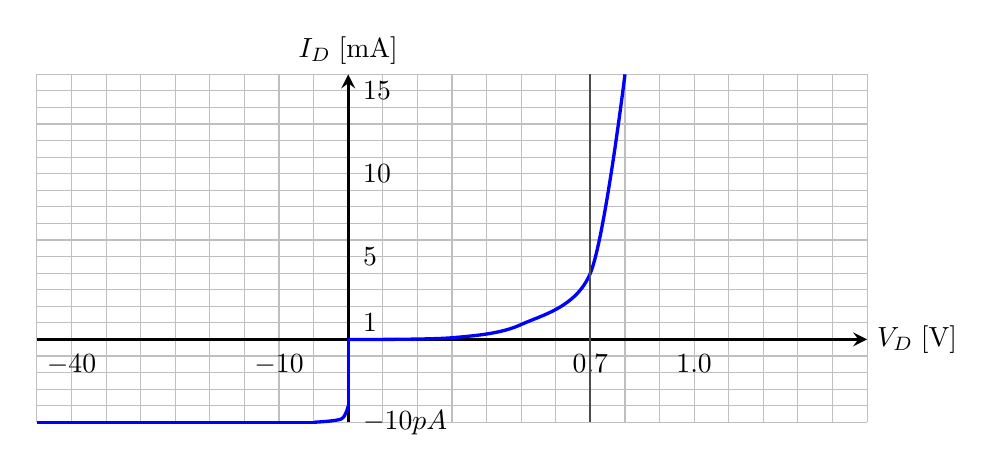
\begin{tikzpicture}
\begin{axis}[
    width=\textwidth,
    height=6cm,
    xmin=-9, xmax=15,
    ymin=-5, ymax=16,
    axis lines=middle,
    axis line style={black, very thick},
    xlabel={$V_D\;[\mathrm{V}]$},
    ylabel={$I_D\;[\mathrm{mA}]$},
    xlabel style={at={(current axis.right of origin)}, anchor=west},
    ylabel style={at={(current axis.above origin)}, anchor=south},
    xtick={-9,-8,...,15},
    xticklabels={
    {}, $-40$, {}, {}, {}, {}, {}, $-10$, {}, $0$,
    {}, {}, {}, {}, {}, {}, $0.7$, {}, {}, $1.0$, {}, {}, {}, {}
    },
    ytick={-5,-4,...,16},
    yticklabels={$-10\unit{pA}$, {}, {}, {}, {}, $0$, $1$, {}, {}, {}, $5$, {}, {}, {}, {}, $10$, {}, {}, {}, {}, $15$, {},},
    yticklabel style={xshift=4pt, anchor=west},
    grid=both,
    major grid style={gray!50, line width=0.4pt},
    minor grid style={gray!30, line width=0.2pt},
    tick style={draw=none},
    minor tick num=0,
    enlargelimits=false,
    clip=false
]

\addplot[
    blue,
    very thick,
    smooth
] coordinates {
    (0,0)
    (3,0.1)
    (5,0.9)
    (7,4)
    (8,16)
};

\addplot[
    blue,
    very thick,
    smooth
] coordinates {
    (-1,-5)
    (-0.2, -4.8)
    (0,-4)
};

\addplot[
    blue,
    very thick
] coordinates {
    (-9,-5)
    (-1,-5)
};

\addplot[
    blue,
    very thick
] coordinates {
    (0,-4)
    (0,0)
};

\draw[black!70, thick] (axis cs:7,-5) -- (axis cs:7,16);

\end{axis}
\end{tikzpicture}
\caption{Reell diodekarakteristikk}
\end{subfigure}

\caption{Sammenligning mellom idealisert og reell diodekarakteristikk.}
\label{fig:diode_karakteristikk_sammenligning}

\end{figure}

\noindent
Vi kan tydelig se hvordan teoretiske beregninger ikke vil samsvare helt med praktiske målinger. Derfor er mange av avvikene i resultatene forventet. For eksempel, i klippekretsene, regner vi teoretisk at utgangssignalet skal klippes ved $0.7\text{V}$, men i praksis kan det være lavere eller høyere avhengig av strømmen gjennom dioden. Tar vi krets 1 og 2 som eksempel, så klippes utgangssignalet ved $800\text{mV}$, noe som må bety i praksis at det går høyere strøm gjennom dioden. I tillegg ser vi at den idealiserte kurven ikke tar hensyn til negativ påført spenning, men som vi ser i den reelle karakteristikken, vil det være en liten lekkasjestrøm i revers retning. I likeretterkretsene, gir resultatene en del avvik i ekstremalpunktene. Dette kan også forklares i den idealiserte modellen. Teoretisk forventer vi at det skal være et spenningsfall på $1.4\text{V}$ over to dioder, men i praksis har vi et spenningsfall på omtrent $2\text{V}$, noe som indikerer at det er høyere strøm gjennom diodene enn det den idealiserte modellen forutsetter. Samlet sett er det viktig å erkjenne at den idealiserte diodemodellen har begrensninger, og at avvik mellom teori og praksis i stor grad kan forklares ved å ta hensyn til de faktiske karakteristikkene til dioden.

\paragraph{Toleranser i komponenter. } Alle komponenter som brukes i eksperimentet har en viss toleranse, noe som betyr at deres faktiske verdier kan avvike fra de nominelle verdiene. For eksempel, motstanden på $180\Omega$ kan ha en toleranse på $\pm 5\%$, noe som betyr at den faktiske motstanden kan være mellom $171\Omega$ og $189\Omega$. Dette kan påvirke strømmen betydelig for vår del, og dermed påvirke arbeidspunktet til dioden. Dette vil føre til at resultatene kommer til å avvike fra de teoretiske beregningene. For eksempel, i klippekretsene, vil motstandsverdien direkte påvirke på hvilken spenning utgangssignalet klippes. Dersom motstanden er lavere enn forventet, vil det være høyere strøm gjennom dioden, noe som kan føre til at klippeverdien er høyere enn det den idealiserte modellen forutsetter. Toleransen i motstanden er derfor i dette forsøket, med på å kunne forklare noe avviket i kretsene. I tillegg, vil den praktiske dioden også ha en viss variasjon i sine karakteristikker. Alt i alt er toleranser i komponenter en viktig feilkilde som kan bidra til avvik mellom teoretiske forventninger og praktiske målinger.

\paragraph{Jordingsfeil. } Ved bruk av måleinstrumenter som oscilloskop og signalgenerator, vil vi introdusere jordingsnoder i kretsen. I toveis likeretter er dette et tilfelle av uønskede slike jordingsnoder. Denne feilkilden førte til helt uforventede resultater i krets 5, der utgangssignalet oppførte seg som en positiv enveis likeretter i stedet for en toveis likeretter. Dette skyldes at kretsen blir forandret og vi kortslutter to noder i kretsen til jording, strømmen går ikke som forventet, og resultatene blir helt annerledes. Uansett, fikser vi denne feilkilden ved å bruke en transformator for å oppnå galvanisk isolasjon, og da får vi resultater som er i god overensstemmelse med teorien. Jordingsfeil er derfor en kritisk feilkilde som kan ha stor innvirkning på resultatene, og det er viktig å være oppmerksom på ved videre oppsett av kretser og måleinstrumenter.

\paragraph{Instrumenter. } Funksjonsgeneratoren og oscilloskopet er ikke noe vi tar hensyn til i de teoretiske utregningene, siden de er antatt å være perfekte. I praksis har de imidlertid begrensninger og kan introdusere støy og andre feil i målingene. For eksempel, oscilloskopet kan ha en viss inngangsimpedans som påvirker kretsen, og det kan også introdusere støy i signalet. I tillegg vil den ikke kunne vise signalene perfekt på skjermen, og resultatgrafene er derfor ikke helt nøyaktige. Funksjonsgeneratoren kan også ha en viss utgangsimpedans og kan introdusere støy i signalet. Disse faktorene påvirket derimot ikke resultatene i noen av kretsene i særlig grad, og de kan derfor anses som mindre feilkilder sammenlignet med de andre nevnte feilkildene.

\subsection{Mulige bruksområder}
Dioder brukes i en rekke elektroniske anvendelser. En av de viktigste er likeretterkretser, hvor vekselspenning omformes til likespenning, for eksempel i strømforsyninger til elektronisk utstyr. Videre benyttes dioder til spenningsbeskyttelse, som ved feil polaritet i batterikretser eller som overspenningsvern (zenerdioder) i følsom elektronikk. Dioder brukes også i signalbehandling, hvor de kan klippe eller forskyve spenningssignaler, slik som i enkle bølgeformingskretser. Generelt sørger dioder for at strøm kun går i én retning i en krets, noe som blant annet utnyttes i strømstyring mellom flere spenningskilder.

\subsection{Forbedringer og videre arbeid}
En viktig forbedring i dette forsøket ville vært å sikre korrekt jording i oppkoblingen fra start. Som observert i krets 5 førte jordingsfeil til at måleresultatene avvek betydelig fra teorien. Ved å benytte galvanisk isolasjon, for eksempel gjennom bruk av transformator, kan slike feil unngås og mer pålitelige målinger oppnås.
\\[1em]
For videre arbeid kunne det vært interessant å undersøke hvordan endringer i frekvens og belastning påvirker rippel og DC-verdi i likeretterkretser med kondensator. I tillegg kunne en mer detaljert analyse av diodens karakteristiske kurve, for eksempel ved å måle strøm-spenningsforholdet direkte, gitt en dypere forståelse av avvikene mellom idealisert og virkelig oppførsel.